% Niveau :      PCSI *
% Discipline :  Chimie Orga I
% Mots clés :   Spectrométrie UV-visible, Réactions acidobasiques

\begin{exercise}{Précipitation sélective}{2}{PCSI}
{Chimie générale,Réactions de précipitation, Solubilité, Précipitation sélective}{bermu}

Actuellement, les métaux présents dans les effluents liquides industriels sont précipités sous forme de boues d'hydroxydes métalliques qui sont stockées comme déchets ultimes sans possibilité de valorisation. Nous allons étudier une alternative écologique consistant à les précipiter sélectivement pour les séparer et les revaloriser.

\begin{questions}
\questioncours Paramètres influençant la solubilité des sels en solution aqueuse. \\
On donnera les tendances générales et on illustrera d'exemples.

\begin{EnvUplevel}
    On considère tout d'abord le cas de l'aluminium. L'hydroyde d'aluminium $\mathrm{{Al{(OH)}_3}_{(s)}}$ est un solide formé par les équilibres successifs suivants :
    $$\mathrm{{Al^{3+}}_{(aq)} + 4 {OH^-}_{(aq)} \overset{\mathnormal{K_s} = 10^{-32}}{\leftrightharpoons} {Al{(OH)}_3}_{(s)} + {OH^-}_{(aq)}  \overset{\mathnormal{K_f} = 10^2}{\leftrightharpoons} {[Al{(OH)}_4]^-}_{(aq)}}.$$
    
    On considérera la quantité globale en aluminium fixée à [Al]$_\text{tot} = 10^{-2}$ mol$\cdot$L$^{-1}$.
\end{EnvUplevel}

\question \'Ecrire le produit de solubilité $K_{s,\mathrm{{Al{(OH)}_3}}}$ et donner le critère de précipitation de $\mathrm{{Al{(OH)}_3}_{(s)}}$.

\question Quel est le comportement acido-basique $\mathrm{{Al{(OH)}_3}_{(s)}}$ ? \\ Calculer les pH d'apparition pH$_a$ et de disparition pH$_d$ de $\mathrm{{Al{(OH)}_3}_{(s)}}$ puis tracer le diagramme d'existence de cet hydroxyde en fonction du pH.

\question Tracer qualitativement $\log s$ en fonction du pH, $s$ étant la somme des concentrations des espèces de l'aluminium solubles. \\
On veillera bien à distinguer les différents cas vus à la question précédente.

\question Quel est le pH optimal pH$^\ast$ pour précipiter  $\mathrm{{Al{(OH)}_3}_{(s)}}$ ?

\begin{EnvUplevel}
    Le problème de la précipitation des hydroxydes est qu'elle est peu sélective et ne permet pas de traiter tous le métaux comme l'illustre la figure ci-dessous : \vspace{-.4em}
    
    \begin{figure}[H]
        \centering
        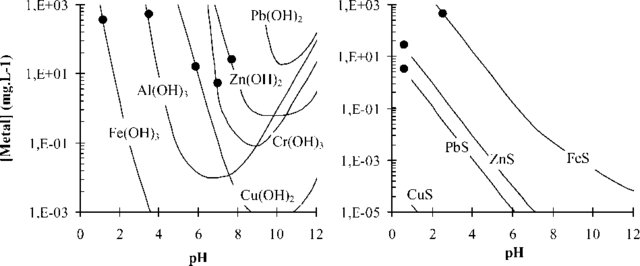
\includegraphics[width=.9\linewidth]{chimie/precipitation/precipitation_selective.png}
        \caption{Solubilités des hydroxydes métalliques et des sulfures métalliques en fonction du pH.}
    \end{figure}
\end{EnvUplevel}

\question Justifier le défaut de sélectivité de la précipitation d'hydroxydes.

\question{\sffamily Question ouverte :} établir un protocole expérimental chiffré pour traiter un mélange d'hydroxydes métalliques industriel en vous aidant de la Fig. 1 et des données ci-dessous. \\
On pourra commencer par un mélange contenant uniquement de l'aluminium et du cuivre par exemple.

\end{questions}

\paragraph{Données :} masses molaires (g$\cdot$mol$^{-1}$) \vspace{-1em}

\begin{table}[H]
    \centering
    \begin{tabularx}{0.8\linewidth}{CCCCCCCCCCCC}
        H   & O  & Na & Al & S  & Cr & Fe & Cu & Zn & Pb \\ \hline
        1,0 & 16 & 23 & 27 & 32 & 52 & 56 & 64 & 66 & 82 \\ \hline\hline
    \end{tabularx}
\end{table}

\plusloin Marina Maya Marchioretto emph{et al.} Heavy Metals
Precipitation in Sewage Sludge, \textit{Separation Science and Technology}, Vol. 40, no. 16, \textbf{2005}, 3393--3405. \vspace{-.5em}
\end{exercise}

\begin{solution}
\begin{questions}
    \questioncours
    \begin{itemize}
        \item \emph{Température :} globalement, la solubilité augmente avec la température (question d'entropie). Cela peut être utile pour dissoudre à chaud ou faire de la cristallisation.
        
        \item \emph{Effet d'ion commun :} La présence d'un ion faisant partie du sel (ion commun) déjà présent en solution augmente le quotient de réaction $Q_r$ et donc diminue la solubilité du sel.
        
        \item \emph{Compétition avec d'autres équilibres :} acide-base , complexation... Ces réactions consomment en partie un ion faisant partie du sel ce qui diminue $Q_r$ et augmente la solubilité.
        
        \end{itemize}
    
    \question À l'équilibre, $Q_r = \mathrm{[Al^{3+}][OH^-]^3} = K_s$ : il y a précipitation si $Q_r > K_s$, en deçà, c'est rupture d'équilibre.
    
    \question $\mathrm{{Al{(OH)}_3}_{(s)}}$ est un amphotère, à la fois acide et base. \\
    Pour l'apparition avec le $K_s$ d'après le critère précédent :
    $$K_s = \mathrm{[Al^{3+}][OH^-]^3} \quad \Longleftrightarrow \quad \text{pH}_a = \text{p}K_e - \dfrac{1}{3}\text{p}K_s - \dfrac{1}{3}\log\mathrm{[Al]_{tot}} = 4.$$
    
    De même pour la disparition
    $$K_f = \mathrm{\dfrac{[{Al(OH)_4}^-]}{[OH^-]}} \quad \Longleftrightarrow \quad \text{pH}_d = \text{p}K_e + \text{p}K_f + \log\mathrm{[Al]_{tot}} = 10.$$
    
    Le domaine d'existance de $\mathrm{{Al{(OH)}_3}_{(s)}}$ est donc $4 \leqslant \text{pH} \leqslant 10$.
    
    \question D'après la question précédente, pour $4 \leqslant \text{pH} \leqslant 10$, les deux équilibres sont atteints, donc
    \begin{align*}
        s(\text{pH}) &= \mathrm{[Al^{3+}] + [{Al(OH)_4}^-]} = K_s 10^{-3(\text{pH} - \text{p}K_e)} + K_f 10^{\text{pH} - \text{p}K_e}, \\
        \noalign{que l'on peut réécrire}
        s(\text{pH}) &= \mathrm{[Al]_{tot}}\qty(10^{-3(\text{pH} - \text{pH}_a)} + 10^{\text{pH} - \text{pH}_d}), \\
        \noalign{et donc, asymptotiquement pour pH - pH$_a$ $\ll$ 1}
        \log s(\text{pH}) &= \log\mathrm{[Al]_{tot}} + 3 \text{pH}_a - 3 \text{pH}, \\
        \noalign{et pour pH$_d$ - pH $\ll$ 1}
        \log s(\text{pH}) &= \log\mathrm{[Al]_{tot}} - \text{pH}_d + \text{pH}.
    \end{align*}
    
    \question Le pH optimal pH$^\ast$ est pour
    $$\dv{s}{\text{pH}} = 0 \quad\Longleftrightarrow\quad
    \text{pH}^\ast = \dfrac{1}{4}\log\qty(3 + 10^{3\text{pH}_a + \text{pH}_d}) \simeq \dfrac{3\text{pH}_a + \text{pH}_d}{4} = 5,5,$$
    (c'est l'interception des deux asymptotes).
    
    \question Les droites de solubilité de la Fig. 3.1 se croisent : les précipités se forment en même quantité pour pH $\geqslant 6$. Ainsi, si Fe et Al peuvent être précipités sélectivement, ce n'est pas le cas de Cu, Zn, Cr et Pb.
    
    \question{\sffamily Suggestion de protocole : }  il faut donc utiliser des sulfures pour traiter Cu, Zn ect.
    
    \begin{itemize}
        \item Partant d'une boue d'hydroxyde, on effectue une lixiviation (= acidifiaction) jusqu'à pH $\simeq 2$ avec de l'acide sulfurique par exemple (éviter les halogènes) ;
        \item Ensuite on rajoute de la soude jusqu'à pH $\simeq 3$ : Fe précipite. Filtrage, lavage, séchage ;
        \item Ensuite on rajoute de la soude jusqu'à pH $\simeq 5,5$ : Al précipite. Filtrage, lavage, séchage ;
    \end{itemize}
    A partir de cet instant, on ne peut plus être sélectif en ajoutant de la soude... On ajoute donc du sulfure de sodium Na$_2$S qui va faire précipier d'abord le Cu, puis le Pb, puis le Zn...
    
\end{questions}
\end{solution}